\documentclass[tikz]{standalone}

\usepackage{hyperref}
\hypersetup{
  pdfinfo={
    CreationDate={D:20180516090844},
    ModDate={D:20180516090844},
  },
}

\usetikzlibrary{shapes.geometric, arrows}
\tikzstyle{box} = [
  rectangle, minimum width=0.13\textwidth, minimum height=0.13\textwidth,
  text centered, draw=black]
\tikzstyle{empty-box} = [
  rectangle, minimum width=0.13\textwidth, minimum height=0.13\textwidth,
  text width=0.05\textwidth]
\tikzstyle{empty-box-vert} = [
  rectangle, minimum width=0.13\textwidth, minimum height=0.13\textwidth,
  text centered, text height=0.001\textwidth]
\tikzstyle{line} = [draw, -latex']

%% cdb == computed ``delta'' b
\usepackage{ifthen}
\newcommand{\cdb}[1]{
  \ifthenelse{\equal{#1}{1}}
             {\widehat{\partial b}}
             {\widehat{\partial^{#1} b}}
}

\begin{document}
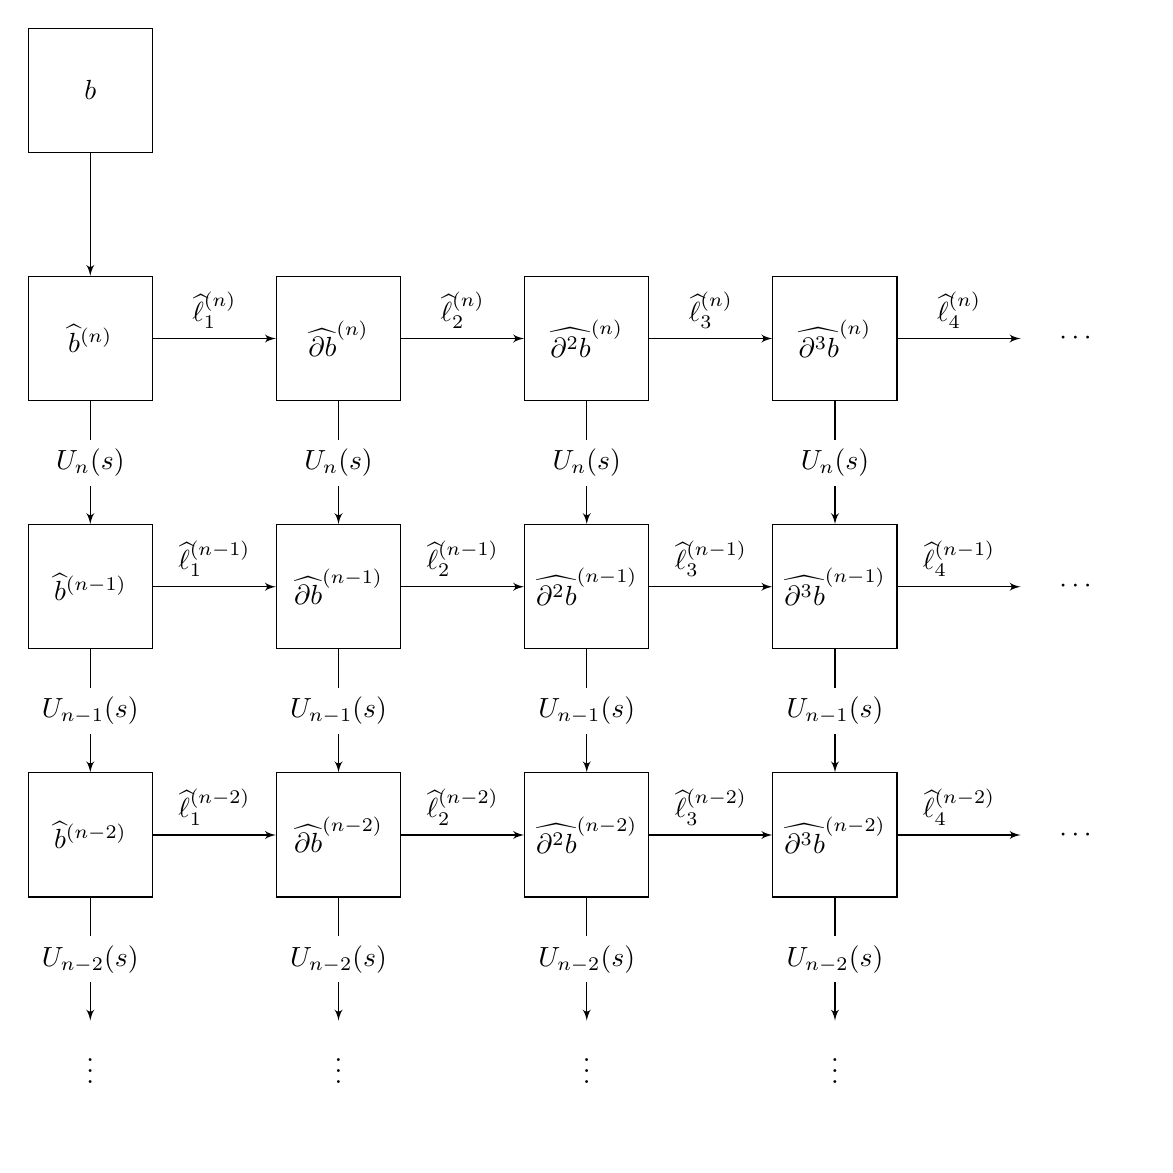
\begin{tikzpicture}[node distance = 0.26\textwidth]
    \node [box] (bj) {\(b\)};
    \node [box, below of=bj] (bn0) {\(\widehat{b}^{(n)}\)};
    \node [box, right of=bn0] (dbn0) {\(\cdb{1}^{(n)}\)};
    \node [box, right of=dbn0] (ddbn0) {\(\cdb{2}^{(n)}\)};
    \node [box, right of=ddbn0] (dddbn0) {\(\cdb{3}^{(n)}\)};
    %%
    \node [box, below of=bn0] (bn1) {\(\widehat{b}^{(n - 1)}\)};
    \node [box, below of=dbn0] (dbn1) {\(\cdb{1}^{(n - 1)}\)};
    \node [box, below of=ddbn0] (ddbn1) {\(\cdb{2}^{(n - 1)}\)};
    \node [box, below of=dddbn0] (dddbn1) {\(\cdb{3}^{(n - 1)}\)};
    %%
    \node [box, below of=bn1] (bn2) {\(\widehat{b}^{(n - 2)}\)};
    \node [box, below of=dbn1] (dbn2) {\(\cdb{1}^{(n - 2)}\)};
    \node [box, below of=ddbn1] (ddbn2) {\(\cdb{2}^{(n - 2)}\)};
    \node [box, below of=dddbn1] (dddbn2) {\(\cdb{3}^{(n - 2)}\)};
    %%
    \path [line] (bn0) -- node[above] {\(\widehat{\ell}_1^{(n)}\)} (dbn0);
    \path [line] (dbn0) -- node[above] {\(\widehat{\ell}_2^{(n)}\)} (ddbn0);
    \path [line] (ddbn0) -- node[above] {\(\widehat{\ell}_3^{(n)}\)} (dddbn0);
    \node [empty-box, right of=dddbn0] (right0) {\(\cdots\)};
    \path [line] (dddbn0) -- node[above] {\(\widehat{\ell}_4^{(n)}\)} (right0);
    %%
    \path [line] (bn1) -- node[above] {\(\widehat{\ell}_1^{(n - 1)}\)} (dbn1);
    \path [line] (dbn1) -- node[above] {\(\widehat{\ell}_2^{(n - 1)}\)} (ddbn1);
    \path [line] (ddbn1) -- node[above] {\(\widehat{\ell}_3^{(n - 1)}\)} (dddbn1);
    \node [empty-box, right of=dddbn1] (right1) {\(\cdots\)};
    \path [line] (dddbn1) -- node[above] {\(\widehat{\ell}_4^{(n - 1)}\)} (right1);
    %%
    \path [line] (bn2) -- node[above] {\(\widehat{\ell}_1^{(n - 2)}\)} (dbn2);
    \path [line] (dbn2) -- node[above] {\(\widehat{\ell}_2^{(n - 2)}\)} (ddbn2);
    \path [line] (ddbn2) -- node[above] {\(\widehat{\ell}_3^{(n - 2)}\)} (dddbn2);
    \node [empty-box, right of=dddbn2] (right2) {\(\cdots\)};
    \path [line] (dddbn2) -- node[above] {\(\widehat{\ell}_4^{(n - 2)}\)} (right2);
    %%
    \path [line] (bj) -- (bn0);
    \path [line] (bn0) -- node[fill=white] {\(U_n(s)\)} (bn1);
    \path [line] (bn1) -- node[fill=white] {\(U_{n - 1}(s)\)} (bn2);
    \node [empty-box-vert, below of=bn2] (bottom0) {\(\vdots\)};
    \path [line] (bn2) -- node[fill=white] {\(U_{n - 2}(s)\)} (bottom0);
    %%
    \path [line] (dbn0) -- node[fill=white] {\(U_n(s)\)} (dbn1);
    \path [line] (dbn1) -- node[fill=white] {\(U_{n - 1}(s)\)} (dbn2);
    \node [empty-box-vert, below of=dbn2] (bottom1) {\(\vdots\)};
    \path [line] (dbn2) -- node[fill=white] {\(U_{n - 2}(s)\)} (bottom1);
    %%
    \path [line] (ddbn0) -- node[fill=white] {\(U_n(s)\)} (ddbn1);
    \path [line] (ddbn1) -- node[fill=white] {\(U_{n - 1}(s)\)} (ddbn2);
    \node [empty-box-vert, below of=ddbn2] (bottom2) {\(\vdots\)};
    \path [line] (ddbn2) -- node[fill=white] {\(U_{n - 2}(s)\)} (bottom2);
    %%
    \path [line] (dddbn0) -- node[fill=white] {\(U_n(s)\)} (dddbn1);
    \path [line] (dddbn1) -- node[fill=white] {\(U_{n - 1}(s)\)} (dddbn2);
    \node [empty-box-vert, below of=dddbn2] (bottom3) {\(\vdots\)};
    \path [line] (dddbn2) -- node[fill=white] {\(U_{n - 2}(s)\)} (bottom3);
\end{tikzpicture}
\end{document}
